%
% -- Manlio Modugno

\documentclass{beamer} 
\usepackage{eulervm}
\usepackage{booktabs}
\usepackage{listings}
\usepackage{bold-extra}
\usepackage{cancel}
\usepackage{fancybox}
\usepackage{soul}
\usepackage[english]{babel}
\usepackage[utf8]{inputenc}
\usepackage{hyperref}
\usepackage{amsmath}
%\hypersetup{colorlinks=true,urlcolor=blue}

\newcommand{\codefont}{\fontsize{6}{8}\selectfont}
\lstset{language=[Sharp]C, 
captionpos=b, 
frame=lines,
lineskip= 1pt, %space between lines
basicstyle=\codefont, 
keywordstyle=\color{blue}, 
commentstyle=\color{green}, 
stringstyle=\color{red}, 
numbers=left, 
numberstyle=\tiny, 
stepnumber=2,
numbersep=5pt,
breaklines=true, 
breakatwhitespace=false,
showstringspaces=false,
frame=single,
tabsize=2,
emph={double,bool,int,unsigned,char,true,false,void},
emphstyle=\color{blue},
emph={Assert,Test},
emphstyle=\color{red},
emph={[2]\using,\#define,\#ifdef,\#endif},
emphstyle={[2]\color{blue}}
}


\mode<presentation>
\definecolor{title_color}{RGB}{2,128,181} 
\usetheme{Ilmenau}
\usecolortheme[named=title_color]{structure}
\setbeamercolor{palette quaternary}{use=structure,fg=black,bg=white} %header footer color
\useoutertheme[subsection=false]{smoothbars}
\setbeamercovered{transparent}
\setbeamertemplate{navigation symbols}{}
\setbeamerfont{subsection in toc}{size=\scriptsize}

\title{Class/Collaboration Diagrams}
\author{Manlio Modugno}
\institute[GMTechnologies] 

\date[16.06.2016] 
{16.06.2016 - Class/Collaboration Diagrams}

\subject{}

\graphicspath{{img/}}
\pgfdeclareimage[height=0.6cm]{mfg-logo}{img/mfgLogo}
\logo{\pgfuseimage{mfg-logo}}

%
% Content start
%
\begin{document}
\begin{frame}
  \titlepage
\end{frame}

\begin{frame}
  \frametitle{Argomenti Trattati}
  \tableofcontents
\end{frame}

\section{UML}
\subsection{Introduction}
\begin{frame}
	\frametitle{Unified Modeling Language}	
	\begin{itemize}
  		\item<+-> It's a visual language for creating models in OO.
		\item<+-> What is a model?  
		\item<+-> ``A conceptual model is a model made of the composition of concepts, which are used to help people know, understand, or simulate a subject the model represents''
		\item<+-> ...we can say: ``something that help us to start to solve a problem..''		
	\end{itemize}
\end{frame}

\subsection{Meta Model}
\begin{frame}
	\frametitle{Meta Model}
	\begin{itemize}
  			\item<+-> It's a standard data representation of UML using UML.
  			\item<+-> Describes the objects, attributes, and relationships necessary to represent the concepts of UML within a software application
	\end{itemize}
\end{frame}

\subsection{Notation}
\begin{frame}
	\frametitle{Notation: two major subdivisions}
	\textbf{Static:}
	\begin{itemize}
  			\item Classes, attributes, relationships, ...
	\end{itemize}
	\textbf{Dynamic:}
	\begin{itemize}
  			\item Objects, messages, finite state machines, ...
	\end{itemize}
\end{frame}

\section{Class Diagrams}
\subsection{Intro}
\begin{frame}
	\frametitle{Class Diagrams(static)}
	\begin{center}
		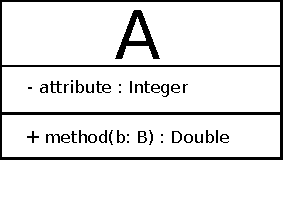
\includegraphics[scale=0.6]{class}
	\end{center}
	\textbf{Note:}
	\begin{itemize}
	\item Attributes and methods can be omitted or can be shown partially
	\item What (usually) really care is to focus on the main concepts
  	\item Focus on a system in general or to a specific part $\Rightarrow$ different diagrams and details
	\item Optional visibility (+ public,\# protected, - private)
	\end{itemize}
\end{frame}

\subsection{Dependency}
\begin{frame}
	\frametitle{Dependency / Relationship}
	\begin{center}
		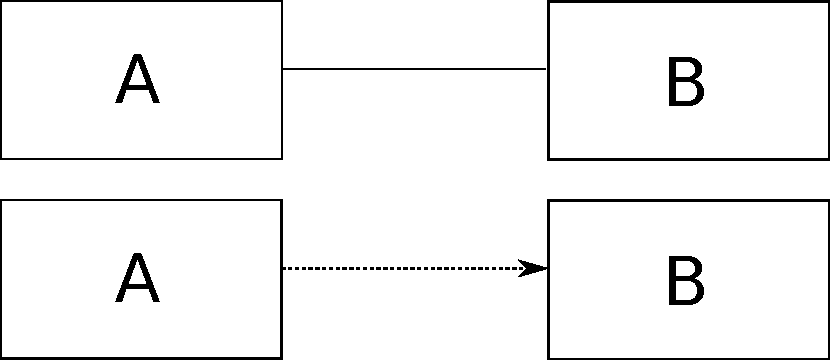
\includegraphics[scale=0.4]{association}
	\end{center}
	\textbf{Note:}
	\begin{itemize}
  			\item Strong / weak (i.e. A somehow depends upon B)
  			\item Uni / Bi directional (default)
  			\item ...
  			\item optional multiplicity (e.g. 0..1, 0..*, etc)
	\end{itemize}
\end{frame}

\subsection{Composition}
\begin{frame}
	\frametitle{Composition Relationships}
	\begin{center}
		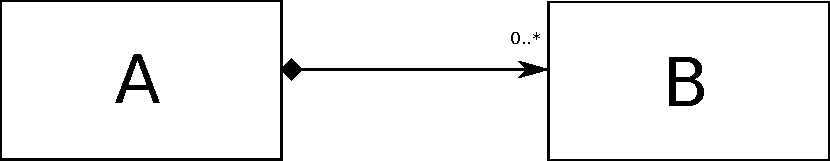
\includegraphics[scale=0.4]{composition}
	\end{center}
	\textbf{Note:}
	\begin{itemize}
  			\item A is composed of a B
  			\item Arrowhead implies one direction navigation (i.e. B can't see A in any way, no import statement)
  			\item It's a strong form of containment or aggregation $\Rightarrow$ lifetime of B is dependent upon A (i.e. If A is destroyed, B is also destroyed)
	\end{itemize}
\end{frame}

\begin{frame}[containsverbatim]
	\frametitle{Translating to code}
	\begin{lstlisting}
class A  
{   
  private Collection<B> _b;

  ...
}
\end{lstlisting}
\end{frame}

\subsection{Aggregation}
\begin{frame}
	\frametitle{Aggregation Relationships}
	\begin{center}
		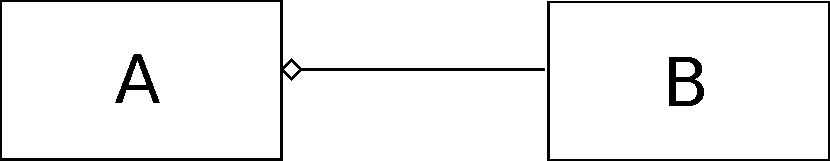
\includegraphics[scale=0.4]{aggregation}
	\end{center}
	\textbf{Note:}
	\begin{itemize}
  			\item A (the aggregate class) is the whole and B is part (of that whole)
  			\item It's a soft form of containment or aggregation
	\end{itemize}
\end{frame}

\subsection{Inheritance}
\begin{frame}
	\frametitle{Inheritance}
	\begin{center}
		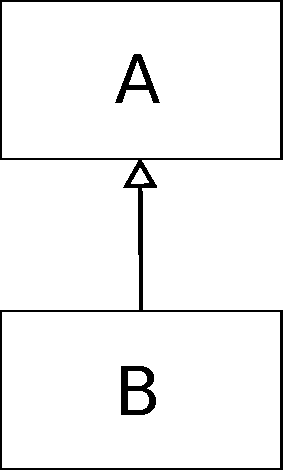
\includegraphics[scale=0.4]{inheritance}
	\end{center}
	\textbf{Note:}
	\begin{itemize}
  			\item Arrohead points to base class
  			\item \textit{Italic fonts} denote abstract class / methods (use \{abstract\} property as alternative)
  			\item \textbf{Warning!}: Inheritance can be dangerous! (LSP and Extends is evil)
	\end{itemize}
\end{frame}

\subsection{Interface}
\begin{frame}
	\frametitle{Interface}
	\begin{center}
		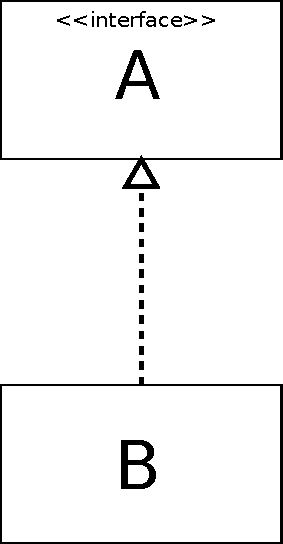
\includegraphics[scale=0.4]{interface}
	\end{center}
	\textbf{Note:}
	\begin{itemize}
  			\item No attributes
  			\item Has only (optionaly depicted) abstract public methods
	\end{itemize}
\end{frame}

\section{Collaboration / Communication) Diagrams}
\subsection{Introduction}
\begin{frame}
	\frametitle{Collaboration / Communication) Diagrams (dynamic)}
	\begin{itemize}
  			\item<+-> UML has different kinds of diagrams that depict dynamic models
  			\item<+-> \textbf{Sequence:} focus on the order in which the messages are sent between objects (procedural flow)
  			\item<+-> \textbf{Collaboration:} focus upon the relationships between objects i.e. the collaboration to get a job done. Usefull also to compare with a static model. 
	\end{itemize}
\end{frame}

\subsection{Interplay between static and dynamic models}
\begin{frame}
	\frametitle{Interplay between static and dynamic models}
	\begin{itemize}
  			\item<+-> \textbf{Static emphasis on object oriented design is inappropriate!}
  			\item<+-> \textbf{Software design is about behavior; and behavior is dynamic!}
  			\item<+-> \textbf{Object oriented design is a technique used to separate and encapsulate behaviors}
  			\item<+-> Interplay between static and dynamic models to prove / refine a solution
	\end{itemize}
\end{frame}

\subsection{Example: A Cellular Phone}
\begin{frame}
	\frametitle{Example: A Cellular Phone}
  		Starting from a static model can be misleading even comparing to real world scenario \\
  		\begin{center}
		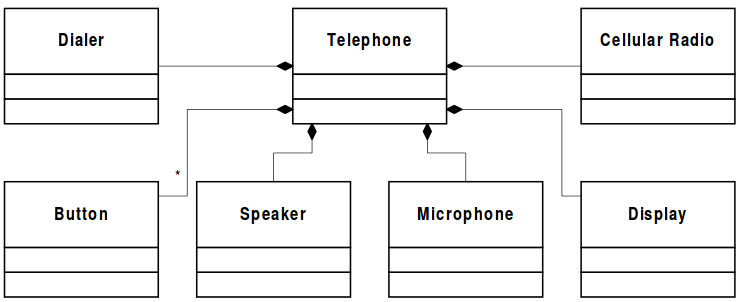
\includegraphics[scale=0.38]{cellStatic}
		\end{center}
\end{frame}

\subsection{Specifying Dynamics}
\begin{frame}
	\frametitle{Specifying Dynamics (with use case / scenario)}
  		\texttt{
  		Use case: Make Phone Call \\
1.User presses the digit buttons to enter the phone number. \\
2.For each digit, the display is updated to add the digit to the
phone number. \\
3.For each digit, the dialer generates the corresponding tone and
emits it from the speaker. \\
4.User presses ``Send'' \\
5.The ``in use'' indicator is illuminated on the display \\
6.The cellular radio establishes a connection to the network. \\
7.The accumulated digits are sent to the network. \\
8.The connection is made to the called party. \\
  		}
\end{frame}

\begin{frame}
	\frametitle{Specifying Dynamics (collaboration)}
	\begin{center}
		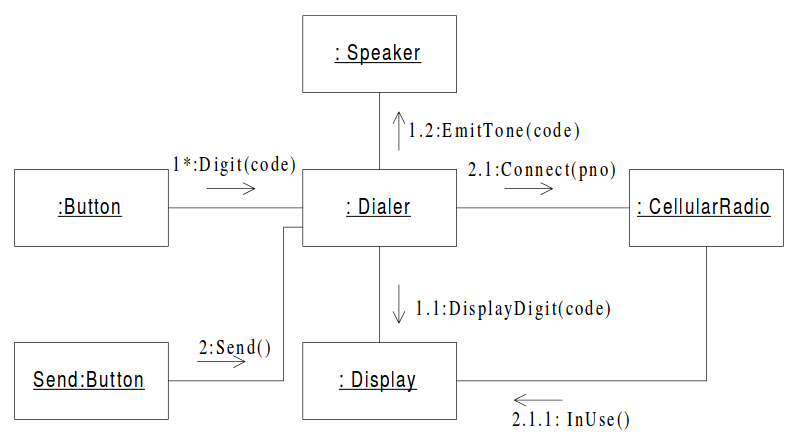
\includegraphics[scale=0.38]{collaboration}
	\end{center}
\end{frame}

\begin{frame}
	\frametitle{Syntax}
	\begin{itemize}
  		\item Rectangles depict objects, not classes
  		\item Object names are optional (i.e. anonymous). They are composite with Class name when present (i.e. Send:Button)
  		\item Lines are called \textit{links}.
	\end{itemize}
\end{frame}

\begin{frame}
	\frametitle{Rules:}
	\begin{itemize}
  		\item Mutual relationship exists between links in collaboration diagram and associations in class diagram.
  		\item Arrows are messages (name, sequence number, arguments). A message name is a method name defined in the class of the receiving object. 
  		\item The sequence numbers show the order in which the messages occur, considering eventual nesting
	\end{itemize}
\end{frame}

\begin{frame}[containsverbatim]
	\frametitle{Translating to code}
	\begin{lstlisting}
class Dialer  {   
  void Send(){  	
  	new CellularRadio().Connect(pno);
  	...
  }
}
class CellularRadio {   
  private Display _diplay;
  
  void Connect(pno){  	
  	_display.InUse();
  	...
  }
  ...
}
class Display  {   
  void InUse(){
  	...
  }
  ...
}
\end{lstlisting}
\end{frame}

\begin{frame}
	\frametitle{Reconciling the static model with the dynamic model}
	\begin{center}
		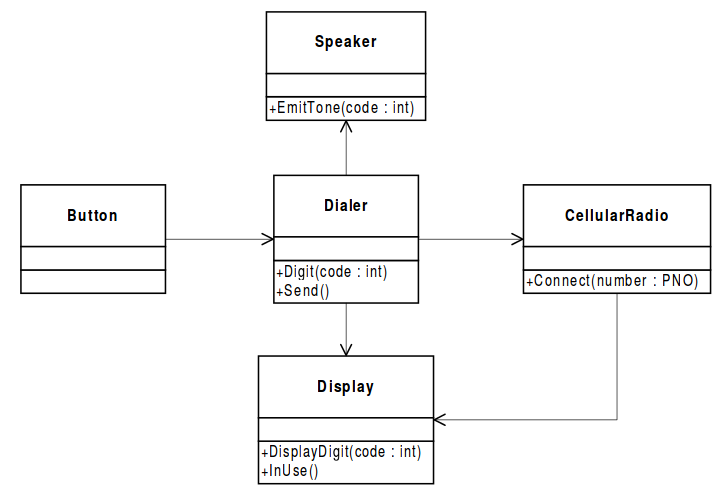
\includegraphics[scale=0.38]{properStatic}
	\end{center}
\end{frame}

\begin{frame}
	\frametitle{Reconciling the static model with the dynamic model}
		\begin{itemize}
		\item Starting from a static model brings to a weird design. ``god'' (i.e. knows everything) object coupled with every other. A rigid and fragile example of design.
  		\item Tha dynamic one encapsulates behaviouh in a proper way. 
  		\item \textbf{Changes to one part of the model do not necessarily impact to other parts}
  		\item \textbf{Pay attention to the ``Real World Guideline''.} Sometime it's not a good clue to follow.. we dive in a behavioral world and some entities don't exist.. (i.e. physical phones vs behavioral one, think to a 'Controller', etc.)
  		\end{itemize}
\end{frame}

\section{Questions}
\begin{frame}
	\frametitle{Questions}
	\begin{itemize}
  			\item ??? 
	\end{itemize}
\end{frame}

\section{Next}
\subsection{Argomento}
\begin{frame}
	\frametitle{Argomento: UML Tutorial: sequence diagram + M.Fowler Refactoring - Chapter 1. Refactoring, a First Example}	

	\begin{itemize}
     		\item studiare \href{http://docs.oracle.com/javase/tutorial/java/concepts/class.html}{Sequence Diagram}
     		\item studiare M.Fowler Refactoring - Chapter 1. Refactoring, a First Example
	\end{itemize}
\end{frame}

\subsection{Esercitazione}
\begin{frame}
\frametitle{Esercitazione}	

\begin{itemize}
	\item Realizzare il class diagram del collaboration presente  \href{http://www.agilemodeling.com/artifacts/communicationDiagram.htm}{qui}
	\item Tradurlo in codice Java 
	\item Provare a realizzare un communication di uno scenario qualsiasi (semplice)
\end{itemize}
\end{frame}
\end{document}